% =====================================================================
%  A Comparative Study of Frequent Itemset Mining on Sparse
%  Transaction Data: Apriori versus FP-growth
%  IEEEtran two-column paper.
%  All experimental numbers are macros in numbers.tex, generated by
%  make_numbers.py from the result CSVs (single source of truth).
%  Table bodies are generated by make_tables.py.
% =====================================================================
\RequirePackage[T1]{fontenc}
\documentclass[journal]{IEEEtran}

\usepackage{mathptmx}
\usepackage{amsmath,amssymb}
\usepackage{graphicx}
\usepackage{booktabs}
\usepackage{url}
\usepackage{flushend}
\usepackage[hidelinks]{hyperref}

\graphicspath{{figs/}}

% ---- float placement quotas: a large float that fails the default 0.7
%      top-fraction test is deferred and can push the whole queue past
%      the references ----
\renewcommand{\topfraction}{0.92}
\renewcommand{\bottomfraction}{0.85}
\renewcommand{\textfraction}{0.06}
\renewcommand{\floatpagefraction}{0.78}
\setcounter{topnumber}{2}
\setcounter{dbltopnumber}{2}
\renewcommand{\dbltopfraction}{0.85}
\setcounter{totalnumber}{3}

\setlength{\emergencystretch}{1em}
\setlength{\floatsep}{11pt plus 3pt minus 2pt}
\setlength{\textfloatsep}{13pt plus 3pt minus 2pt}
\setlength{\intextsep}{11pt plus 3pt minus 2pt}
\makeatletter
\setlength{\@fptop}{0pt}
\makeatother

% Auto-generated by make_numbers.py -- do not edit by hand.
\newcommand{\DSN}{1892}
\newcommand{\RobN}{49}
\newcommand{\DSOcc}{22,300}
\newcommand{\MaxKA}{2}
\newcommand{\MaxKB}{3}
\newcommand{\MaxKC}{4}
\newcommand{\MaxKD}{7}
\newcommand{\ItemsA}{96}
\newcommand{\ItemsB}{335}
\newcommand{\ItemsC}{1,115}
\newcommand{\ItemsD}{6,524}
\newcommand{\RulesA}{5}
\newcommand{\RulesB}{49}
\newcommand{\RulesC}{192}
\newcommand{\RulesD}{6,068}
\newcommand{\ApTimeA}{0.022}
\newcommand{\ApTimeB}{0.098}
\newcommand{\ApTimeC}{0.509}
\newcommand{\ApTimeD}{3.999}
\newcommand{\DSItems}{1990}
\newcommand{\FpTimeA}{0.014}
\newcommand{\FpTimeB}{0.035}
\newcommand{\FpTimeC}{0.097}
\newcommand{\FpTimeD}{0.230}
\newcommand{\RevConf}{0.55}
\newcommand{\RobPass}{27}
\newcommand{\SupPctA}{2}
\newcommand{\SupPctB}{1}
\newcommand{\SupPctC}{0.5}
\newcommand{\SupPctD}{0.2}
\newcommand{\TopConf}{0.92}
\newcommand{\TopLift}{41.44}
\newcommand{\CandTwoA}{4,005}
\newcommand{\CandTwoB}{38,781}
\newcommand{\CandTwoC}{261,726}
\newcommand{\CandTwoD}{1,149,886}
\newcommand{\DSAvgLen}{11.79}
\newcommand{\DSMaxLen}{86}
\newcommand{\DSMinLen}{5}
\newcommand{\FreqTwoA}{6}
\newcommand{\FreqTwoB}{52}
\newcommand{\FreqTwoC}{346}
\newcommand{\FreqTwoD}{3,356}
\newcommand{\KeepTwoA}{0.15}
\newcommand{\KeepTwoB}{0.13}
\newcommand{\KeepTwoC}{0.13}
\newcommand{\KeepTwoD}{0.29}
\newcommand{\MaxLiftA}{9.87}
\newcommand{\MaxLiftB}{41.44}
\newcommand{\MaxLiftC}{50.05}
\newcommand{\MaxLiftD}{473.00}
\newcommand{\RobShare}{55.1}
\newcommand{\SpeedupA}{1.57}
\newcommand{\SpeedupB}{2.81}
\newcommand{\SpeedupC}{5.26}
\newcommand{\SpeedupD}{17.39}
\newcommand{\DSMaxSupp}{10.0}
\newcommand{\LiftBound}{5.0}
\newcommand{\MinCountA}{37.84}
\newcommand{\MinCountB}{18.92}
\newcommand{\MinCountC}{9.46}
\newcommand{\MinCountD}{3.78}
\newcommand{\PyVersion}{3.13.14}
\newcommand{\RevConfHi}{0.68}
\newcommand{\RevConfLo}{0.43}
\newcommand{\RobSupMax}{78}
\newcommand{\RobSupMed}{25}
\newcommand{\RobSupMin}{19}
\newcommand{\TopConfHi}{1.00}
\newcommand{\TopConfLo}{0.84}
\newcommand{\TopLiftHi}{55.65}
\newcommand{\TopLiftLo}{33.78}
\newcommand{\BootstrapB}{200}
\newcommand{\CandTotalA}{5,996}
\newcommand{\CandTotalB}{40,785}
\newcommand{\CandTotalC}{263,951}
\newcommand{\CandTotalD}{1,161,310}
\newcommand{\DSItemsOne}{279}
\newcommand{\KeepTotalA}{1.60}
\newcommand{\KeepTotalB}{0.82}
\newcommand{\KeepTotalC}{0.42}
\newcommand{\KeepTotalD}{0.56}
\newcommand{\RulesLiftA}{5}
\newcommand{\RulesLiftB}{49}
\newcommand{\RulesLiftC}{192}
\newcommand{\RulesLiftD}{6,068}
\newcommand{\TreeDepthA}{22}
\newcommand{\TreeDepthB}{33}
\newcommand{\TreeDepthC}{52}
\newcommand{\TreeDepthD}{73}
\newcommand{\TreeNodesA}{3,205}
\newcommand{\TreeNodesB}{8,019}
\newcommand{\TreeNodesC}{13,824}
\newcommand{\TreeNodesD}{18,851}
\newcommand{\DSItemsFive}{14}
\newcommand{\RobWidthMed}{4.22}
\newcommand{\CandOverTreeD}{61.6}
\newcommand{\DSTopItemCount}{189}
\newcommand{\RulesAConfFifty}{5}
\newcommand{\RulesAConfSixty}{2}
\newcommand{\RulesBConfFifty}{49}
\newcommand{\RulesBConfSixty}{29}
\newcommand{\RulesCConfFifty}{192}
\newcommand{\RulesCConfSixty}{117}
\newcommand{\RulesDConfFifty}{6,068}
\newcommand{\RulesDConfSixty}{4,346}
\newcommand{\RulesAConfSeventy}{0}
\newcommand{\RulesBConfSeventy}{15}
\newcommand{\RulesCConfSeventy}{71}
\newcommand{\RulesDConfSeventy}{2,959}


\begin{document}

\title{Apriori and FP-growth on Sparse Transactions:\\
Computational Cost and Association Rule Stability}

\author{Weixin~Chen% <-this % stops a space
\thanks{Manuscript prepared October 2026.
Course project for Big Data Analysis and Processing, experiment 2.
Code and result files accompany this paper.}}

\markboth{Big Data Analysis and Processing --- Experiment 2, October 2026}%
{Chen: Frequent Itemset Mining on Sparse Transaction Data}

\maketitle


\begin{abstract}
Lowering minimum support uncovers combinations that occur in few baskets. It also expands the search and makes the confidence of individual rules sensitive to a few observations.
We implemented Apriori and FP-growth in Python and compared their outputs and running times on \DSN{} transactions containing \DSItems{} distinct items.
Both algorithms returned identical itemsets and support counts at four thresholds.
Reducing minimum support from \SupPctA\% to \SupPctD\% increased the number of frequent itemsets from \ItemsA{} to \ItemsD{} and widened the observed runtime ratio from \SpeedupA{} to \SpeedupD{} in favour of FP-growth.
Apriori spent most of its time processing pairs and triples at the lowest threshold.
At \SupPctB\% support and 50\% confidence, \RobN{} rules qualified. For \RobPass{} of them, the fifth percentile of bootstrap confidence still met the cutoff. Two rules with identical lift but different antecedents illustrate how this criterion distinguishes the more consistent direction.
\end{abstract}

\begin{IEEEkeywords}
Apriori, association rules, bootstrap, FP-growth, frequent itemsets.
\end{IEEEkeywords}

\section{Introduction}
\IEEEPARstart{I}{n} a sparse transaction database, two items can occur together in nearly every basket containing one of them and still appear in only a small fraction of all baskets. A high support threshold can discard such a pair. Lowering the threshold poses two questions. How much additional work does it take to recover the rarer combinations? Among the rules they yield, which consistently meet the chosen confidence threshold?

Apriori~\cite{agrawal1994} and FP-growth~\cite{han2000} provide a controlled comparison for the first question. Apriori counts explicit candidates at successive itemset lengths. FP-growth stores shared transaction prefixes in a tree and mines conditional patterns. Both seek the same frequent itemsets, so agreement on every support count lets us compare the cost of two search strategies on identical output.

We implemented both miners and a common rule generator, verified their results against a worked example and randomized tests, and recorded per-level candidate counts and elapsed times. For the second question, we evaluated twelve combinations of four support and three confidence thresholds. We then resampled whole transactions to examine how confidence varied for each rule at a selected operating point.

\section{Data and Methods}
The course database contains \DSN{} baskets of integer item identifiers (Table~\ref{tab:data}). A basket contains \DSAvgLen{} items on average. Only \DSItemsOne{} of the \DSItems{} identifiers appear in at least 1\% of baskets. We therefore swept minimum support from \SupPctA\% down to \SupPctD\%. For detailed rule analysis we used \SupPctB\%, which requires at least 19 baskets per itemset and yields a rule set small enough to inspect in full.

\begin{table}[t]
\centering
\caption{Basic statistics of the transaction database.}
\label{tab:data}
\renewcommand{\arraystretch}{1.05}
\begin{tabular}{@{}lr@{}}
\toprule
Quantity & Value\\
\midrule
Transactions & \DSN\\
Distinct items & \DSItems\\
Total item occurrences & \DSOcc\\
Mean transaction length & \DSAvgLen\\
Shortest / longest transaction & \DSMinLen{} / \DSMaxLen\\
Items covering $\ge 5\%$ of transactions & \DSItemsFive\\
Items covering $\ge 1\%$ of transactions & \DSItemsOne\\
\bottomrule
\end{tabular}
\end{table}

\subsection{Mining the Same Itemsets by Two Routes}
For a database of $n$ baskets, let $\sigma(S)$ count the baskets containing every item in $S$. An itemset is frequent if $\sigma(S)\geq\lceil ns\rceil$ for minimum support $s$. The four thresholds in descending order require 38, 19, 10 and 4 baskets, respectively.

Apriori represents each itemset as a sorted tuple. To form a candidate of length $k$, it joins two frequent $(k-1)$-itemsets with a common prefix of length $k-2$ and checks that every immediate subset is frequent. Each surviving candidate enters the support-counting stage. The implementation estimates the number of basket subsets, $\sum_t\binom{|t|}{k}$, and the number of candidate--basket comparisons, $n|C_k|$, where $C_k$ denotes the candidate set after the subset check. It chooses the counting strategy with the smaller estimate. For each level we record $|C_k|$, the number meeting minimum support, and the time for generation and counting together.

FP-growth counts individual items, drops infrequent ones and inserts the remaining items in descending frequency order into a prefix tree. Baskets with a common prefix share nodes. For each suffix item, the miner collects its prefix paths, weights them by their counts and recursively mines the resulting conditional tree. Both miners return itemsets and integer support counts in the same representation.

\subsection{Implementation Checks and Timing}
We first reproduced the four-basket course example~\cite{notes2026}. At 50\% support, six candidate pairs yield four frequent pairs. Only one triple, $\{2,3,5\}$, survives. The example also checks rule direction. Both baskets containing item~1 contain item~3, whereas only two of the three baskets containing item~3 contain item~1.

We compared Apriori against exhaustive enumeration on 30 randomized databases at four thresholds each. A second test compared FP-growth with Apriori on 25 randomized databases at four thresholds each. The 23 automated tests also cover subset pruning and threshold boundaries. On the course database, we compared the complete itemset-to-count mappings at all four support thresholds.

The single-threaded Python \PyVersion{} benchmark timed the mining calls on the same loaded baskets. If the first call took less than 0.8\,s, the driver reported the minimum of three runs. Otherwise it retained the first time. Per-level measurements come from the first Apriori call. Rule generation and file export were outside the timers.

\subsection{Rule Generation and Resampling}
For every frequent itemset with at least two items, we enumerate each nonempty proper subset $Y$ as an antecedent and use the remaining items $X$ as its consequent. Writing $p(S)=\sigma(S)/n$, the two measures for $Y\to X$ are
\begin{align}
\mathrm{conf}(Y\to X)&=p(X\cup Y)/p(Y),\\
\mathrm{lift}(Y\to X)&=\mathrm{conf}(Y\to X)/p(X).
\end{align}
We retain rules at confidence thresholds of 50\%, 60\% and 70\%. At the working setting of \SupPctB\% support and 50\% confidence, we hold the selected rules fixed. Each of \BootstrapB{} bootstrap replicates draws $n$ whole baskets with replacement and recomputes the measures. The 5th and 95th percentiles form a central 90\% bootstrap interval. Our stability criterion asks whether the lower confidence endpoint reaches 50\%.

\section{Results and Discussion}
\subsection{Lower Support Widens the Runtime Gap}
Table~\ref{tab:levels} compares elapsed time for identical outputs. As minimum support fell from \SupPctA\% to \SupPctD\%, the miners recovered \ItemsD{} itemsets instead of \ItemsA{}, including patterns as long as \MaxKD{} items. FP-growth took less time at each threshold. At \SupPctA\%, the difference was eight milliseconds. At \SupPctD\%, Apriori took \ApTimeD\,s and FP-growth took \FpTimeD\,s, a \SpeedupD-fold difference.

\begin{table}[t]
\centering
\caption{Effect of the support threshold on scale and cost
for the two miners.}
\label{tab:levels}
\renewcommand{\arraystretch}{1.05}
\begin{tabular}{@{}lrrrr@{}}
\toprule
$\mathit{min\_sup}$ & Itemsets & $k_{\max}$ & Apriori (s) & FP-growth (s)\\
\midrule
\SupPctA\% & \ItemsA & \MaxKA & \ApTimeA & \FpTimeA\\
\SupPctB\% & \ItemsB & \MaxKB & \ApTimeB & \FpTimeB\\
\SupPctC\% & \ItemsC & \MaxKC & \ApTimeC & \FpTimeC\\
\SupPctD\% & \ItemsD & \MaxKD & \ApTimeD & \FpTimeD\\
\bottomrule
\end{tabular}
\end{table}

Fig.~\ref{fig:length} shows which pattern lengths account for the larger output. At 1\% support only four triples qualify. At 0.2\%, the output includes 1,255 triples and 324 four-item sets, alongside a single seven-item set. Lower support therefore expands the search across both pairs and longer patterns.

\begin{figure}[t]
\centering
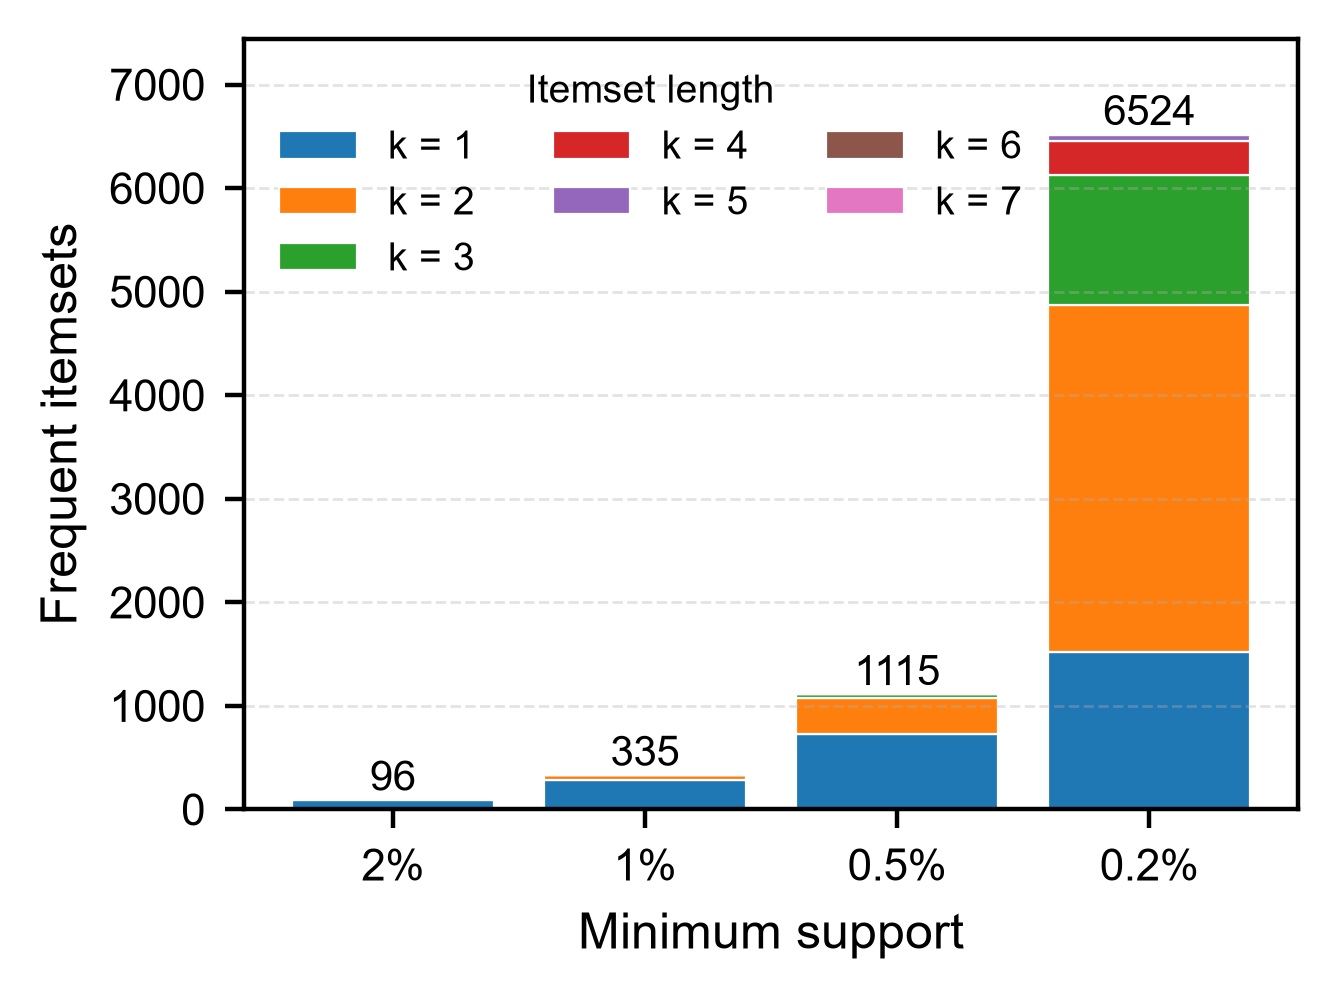
\includegraphics[width=.92\columnwidth]{fig_itemsets.png}
\caption{Frequent itemsets by length. Each bar represents one support threshold, with the total shown above it.}
\label{fig:length}
\end{figure}

Table~\ref{tab:cand} identifies the expensive levels. At 0.2\% support, 1,517 frequent singletons gave Apriori \CandTwoD{} possible pairs. Every pair of frequent singletons passes the subset check, yet only \FreqTwoD{} pairs met the support threshold. Across levels, \ItemsD{} of \CandTotalD{} counted candidates were frequent (\KeepTotalD\%). This percentage measures retention after support counting.

The pair and triple levels took 2.057 and 1.650\,s, respectively, or about 93\% of the recorded level time together. The triple level took nearly as long as the pair level despite admitting far fewer candidates to counting. FP-growth represented the filtered baskets in a main tree with \TreeNodesD{} nodes at this threshold and mined extensions through conditional trees.

\begin{table}[t]
\centering
\caption{Per-level candidates, retained itemsets and time for the working
threshold B ($1\%$) and the stress threshold D ($0.2\%$).}
\label{tab:cand}
\renewcommand{\arraystretch}{1.05}
\begin{tabular}{@{}llrrr@{}}
\toprule
Level & $k$ & Candidates & Retained & Time (s)\\
\midrule
B & 1 & 1,990 & 279 & 0.004 \\
B & 2 & 38,781 & 52 & 0.085 \\
B & 3 & 14 & 4 & 0.009 \\
D & 1 & 1,990 & 1,517 & 0.005 \\
D & 2 & 1,149,886 & 3,356 & 2.057 \\
D & 3 & 8,891 & 1,255 & 1.650 \\
D & 4 & 471 & 324 & 0.263 \\
D & 5 & 62 & 62 & 0.018 \\
D & 6 & 9 & 9 & 0.003 \\
D & 7 & 1 & 1 & 0.002 \\
\bottomrule
\end{tabular}

\end{table}

\subsection{Support Controls Which Rules Enter the Analysis}
Table~\ref{tab:rules} separates the effects of support and confidence. At 50\% confidence, reducing support from 2\% to 1\% raised the rule count from \RulesA{} to \RulesB{}. At 0.2\% support, \RulesD{} rules qualified, and \RulesDConfSeventy{} still qualified at 70\% confidence. At the 2\% support threshold, no rule reached 70\% confidence.

\begin{table}[t]
\centering
\caption{Number of association rules by parameter setting. Every rule in this
table satisfies $\mathrm{lift}>1$.}
\label{tab:rules}
\renewcommand{\arraystretch}{1.05}
\begin{tabular}{@{}lrrr@{}}
\toprule
$\mathit{min\_sup}$ & $50\%$ & $60\%$ & $70\%$\\
\midrule
\SupPctA\% & \RulesA & \RulesAConfSixty & \RulesAConfSeventy\\
\SupPctB\% & \RulesB & \RulesBConfSixty & \RulesBConfSeventy\\
\SupPctC\% & \RulesC & \RulesCConfSixty & \RulesCConfSeventy\\
\SupPctD\% & \RulesD & \RulesDConfSixty & \RulesDConfSeventy\\
\bottomrule
\end{tabular}
\end{table}

The most frequent item appeared in \DSTopItemCount{} of \DSN{} baskets. By subset containment, every nonempty consequent has support at most $\DSTopItemCount/\DSN$. A rule with confidence at least 0.50 therefore has lift at least $0.50/(\DSTopItemCount/\DSN)\approx\LiftBound$. This bound explains why the lift-above-one filter retains every rule in Table~\ref{tab:rules}.

At 0.2\% support, one rule attaining the maximum lift of 473 was $\{30,1546\}\to\{1430,1541\}$. Its antecedent and consequent each occurred in the same four baskets. Confidence was therefore one, and lift was $1/(4/\DSN)=473$. Reporting the four baskets alongside the ratio makes its scale interpretable.

\subsection{Rule Direction Changes the Stability Decision}
At the working setting, joint support ranged from \RobSupMin{} to \RobSupMax{} baskets, with a median of \RobSupMed{}. Among the \RobN{} selected rules, \RobPass{} (\RobShare\%) retained a lower confidence endpoint of at least 50\%. Table~\ref{tab:robust} gives both measures for the eight highest-lift rules.

\begin{table}[t]
\centering
\caption{Strongest rules at the working threshold with 90\% bootstrap
intervals ($B=\BootstrapB$).}
\label{tab:robust}
\renewcommand{\arraystretch}{1.05}
\setlength{\tabcolsep}{3pt}
\begin{tabular}{@{}ccrccrc@{}}
\toprule
$Y$ & $X$ & supp & conf & 90\% CI & lift & 90\% CI\\
\midrule
$\{86\}$ & $\{27\}$ & 0.0122 & 0.92 & [0.84, 1.00] & 41.4 & [33.8, 55.6] \\
$\{27\}$ & $\{86\}$ & 0.0122 & 0.55 & [0.43, 0.68] & 41.4 & [33.8, 55.6] \\
$\{185\}$ & $\{57\}$ & 0.0111 & 0.70 & [0.54, 0.82] & 34.0 & [25.8, 44.7] \\
$\{57\}$ & $\{185\}$ & 0.0111 & 0.54 & [0.39, 0.68] & 34.0 & [25.8, 44.7] \\
$\{44\}$ & $\{55\}$ & 0.0153 & 0.63 & [0.50, 0.76] & 29.8 & [24.1, 38.2] \\
$\{55\}$ & $\{44\}$ & 0.0153 & 0.72 & [0.61, 0.83] & 29.8 & [24.1, 38.2] \\
$\{79\}$ & $\{17\}$ & 0.0122 & 0.57 & [0.46, 0.69] & 25.9 & [20.7, 33.5] \\
$\{17\}$ & $\{79\}$ & 0.0122 & 0.55 & [0.41, 0.67] & 25.9 & [20.7, 33.5] \\
\bottomrule
\end{tabular}

\end{table}

Fig.~\ref{fig:interval} shows the spread of lift estimates among the twelve highest-ranked rules. The two directions of the leading pair have the same interval, a consequence of the symmetry of lift. Their confidence estimates reveal a distinction that the lift plot conceals.

\begin{figure}[t]
\centering
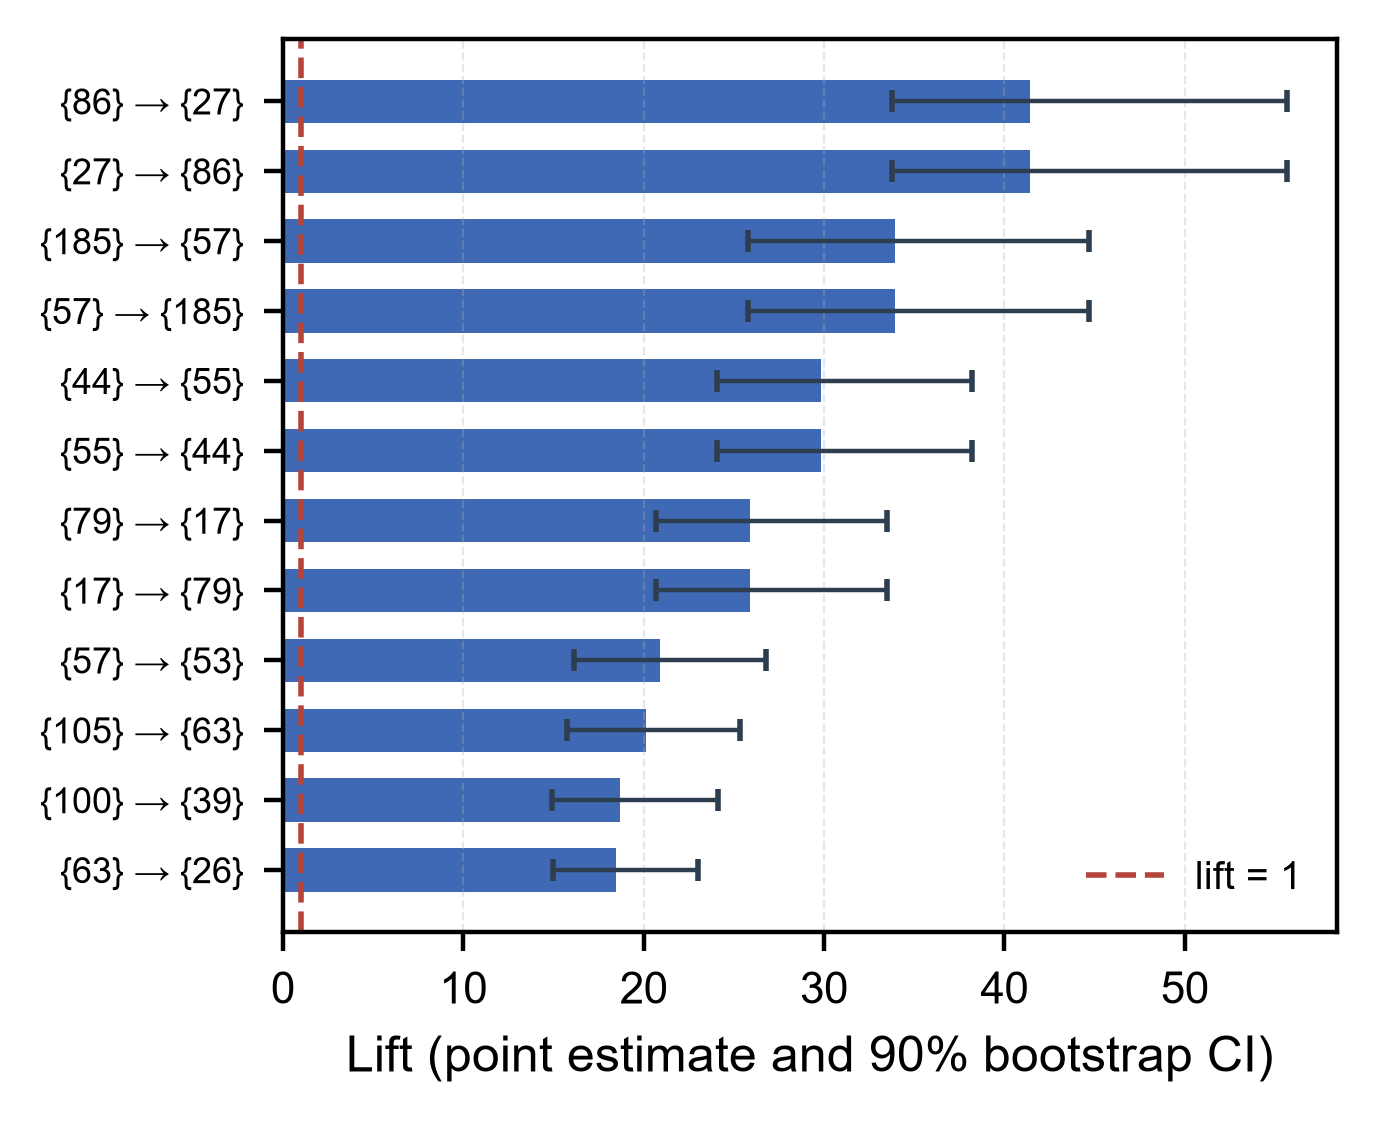
\includegraphics[width=.92\columnwidth]{fig_robust.png}
\caption{Lift and central 90\% bootstrap intervals for the twelve highest-lift rules at 1\% support and 50\% confidence.}
\label{fig:interval}
\end{figure}

Items 86 and 27 shared 23 baskets. Of the 25 baskets containing item~86, 23 also contained item~27, giving confidence \TopConf{}. Reversing the rule changed the denominator to 42 and reduced confidence to \RevConf{}. Both directions had lift \TopLift{} and the same bootstrap lift interval $[\TopLiftLo,\TopLiftHi]$. Their confidence intervals were $[\TopConfLo,\TopConfHi]$ and $[\RevConfLo,\RevConfHi]$, respectively. Both directions met the cutoff in the observed baskets, but only $86\to27$ retained it at the lower bootstrap endpoint. The antecedent count and confidence interval thus distinguish two rules that lift ranks equally.

\section{Conclusion and Future Work}
On \DSN{} sparse transactions, Apriori and FP-growth agreed on every frequent itemset and support count. FP-growth's observed runtime advantage grew from \SpeedupA-fold to \SpeedupD-fold as support fell. Apriori's level timings locate most of the work at pairs and triples. The rule analysis shows what the extra search yields: thousands of low-support rules, some with high lift based on just four baskets. At the 1\% working threshold, bootstrap confidence narrowed \RobN{} rules to \RobPass{} that retained the directional confidence threshold at the lower endpoint.

A follow-up benchmark could vary basket density and repeat each timing under a common protocol, recording candidate generation, counting and peak memory separately. A labelled transaction dataset with timestamps would also allow the rules selected by resampling to be evaluated on later baskets and interpreted in terms of the items involved.

\phantomsection\label{sec:refs}
\begin{thebibliography}{4}

\bibitem{agrawal1994}
R.~Agrawal and R.~Srikant, ``Fast algorithms for mining association rules,''
in \emph{Proc. 20th Int. Conf. Very Large Data Bases}, Santiago, Chile, 1994,
pp.~487--499.

\bibitem{han2000}
J.~Han, J.~Pei, and Y.~Yin, ``Mining frequent patterns without candidate
generation,'' in \emph{Proc. ACM SIGMOD Int. Conf. Management of Data},
Dallas, TX, USA, 2000, pp.~1--12.

\bibitem{notes2026}
\emph{Apriori to Students Homework Readme}, Big Data Analysis and Processing,
Experiment 2, course handout.
\end{thebibliography}
\end{document}
